\section{Experiments}
\label{sec:exp}

\subsection{Experimental Setup}
\paragraph{Benchmarks.}
\emph{ZTF-BTS} is FLARE's public Bright Transient Survey benchmark \citep{fremling2020bts,perley2020bts,sasli2026forecast,sasli2026flare} (10,492 spectroscopically classified transients with future targets across six classes), evaluated using FLARE's prefix-causal features, relative $g$/$r$ magnitude targets up to 90 days, five origins ($5,10,15,20,30$d), and five stratified folds.
\emph{PLAsTiCC-train} (2,045 objects, 11 classes) and \emph{PLAsTiCC-DDF} (8,681 chunk-01 deep-drilling objects, 9 classes) come from the unblinded LSST simulation \citep{kessler2019models,hlozek2023results} at origins $5,15,30$d.
Three UCR archives \citep{dau2019ucr}---StarLightCurves (9,236, 3 classes), ECG5000 (5,000, 5 classes, smallest 24), and ElectricDevices (16,637, 7 classes)---are forecast from $20\%,40\%,60\%$ prefixes (\cref{tab:bench}), with UCR Wafer (20\%) and a synthetic suite in the appendix.
Main experiments follow FLARE's five-fold cross-conformal protocol, calibrating on four out-of-fold sets and pooling test predictions across all five folds.

\paragraph{Models and Baselines.}
Every method shares identical cross-fitted classifiers (FLARE's hierarchical model on ZTF; class-weighted LightGBM elsewhere) and LightGBM quantile forecasters \citep{ke2017lightgbm} (\cref{app:protocol}), isolating conformal calibration.
We evaluate 13 external baselines across four families (\cref{app:baselines}):
\emph{Deployed:} FLARE's predicted-class Mondrian bands \citep{sasli2026forecast,sasli2026flare};
\emph{Membership-blind:} normalised-residual split CP \citep{lei2018distribution}, CQR \citep{romano2019conformalized}, and DCP \citep{chernozhukov2021distributional};
\emph{Probability-conditioned:} Localized CP \citep{guan2023localized}, label-shift mixture \citep{podkopaev2021distribution}, GCC \citep{gibbs2025conformal}, learned-partition CP \citep{kiyani2024conformal}, and CPTC \citep{sun2025conformal};
\emph{Latent-class-valid:} two-step CP \citep{timans2024adaptive}, Kandinsky CP \citep{bairaktari2025kandinsky}, MDCP \citep{yang2026multi}, and max-class CP \citep{barber2021limits}.
CPTC, Kandinsky CP, and MDCP use our \textbf{C1} forecaster; we also test \emph{+\,C1} variants of two-step, MDCP, and max-class CP, plus an oracle \emph{True-class Mondrian} reference.

\paragraph{Metrics.}
We report point-pooled class coverage, object-level per-(class, bin) coverage (\cref{eq:target}), worst-class coverage, $\mathrm{CCG}=\frac1K\sum_c|\mathrm{cov}_c-(1-\alpha)|$, and mean width relative to FLARE.
A setting is \emph{valid} if every class's 95\% object-level bootstrap upper bound (500 resamples) reaches $1-\alpha$.
Our initial plan (\cref{app:plan}) pre-registered a fixed worst-class tolerance ($\ge$ nominal $-0.02$/$-0.015$; \cref{app:results}) and class-averaged interval score \citep[IS;][]{gneiting2007strictly}: on IS, \gamut{} ranks first among all valid methods in \ISWinsGamutSixtyeight{} (68\%) and \ISWinsGamutNinetyfive{} (95\%) settings, while beating each always-valid baseline in paired bootstrap tests far more often than losing (two-step \ISVsTwoStepGamutSixtyeight{}, \ISVsTwoStepGamutNinetyfive{}; max-class \ISVsMaxClassGamutSixtyeight{}, \ISVsMaxClassGamutNinetyfive{}; MDCP \ISVsMDGamutSixtyeight{}, \ISVsMDGamutNinetyfive{}; \cref{app:unfavourable}). Main tables report width, matching \cref{prop:oracle}.

\subsection{Main Quantitative Comparison}
\begin{table*}[t]
\centering
\caption{Aggregate performance across the six main benchmarks and all forecast origins (20 settings per nominal level). \emph{Valid}: percentage of settings with no significantly under-covered class (95\% object-level bootstrap upper bound $\ge 1-\alpha$). \emph{Worst}: mean worst-class coverage across settings. \emph{CCG}: mean absolute class-coverage gap. \emph{Cells}: mean number of significantly under-covered (class, lead-time bin) cells per setting. \emph{Width}: mean band length relative to deployed FLARE. Rows are grouped into deployed/membership-blind, probability-conditioned, latent-class-valid, controlled \emph{+\,C1} variants, and \gamut{}. Boldface highlights the best metric among methods achieving $\ge90\%$ empirical class validity at that level. Under this cross-fitted protocol, \emph{\gamut{} (split calibration)} is empirical; formal finite-sample certification requires the strict split in \cref{tab:strictsum,tab:strict}.}
\label{tab:main}
\small
\setlength{\tabcolsep}{5pt}
\resizebox{\linewidth}{!}{%
\begin{tabular}{lccccc@{\hspace{12pt}}ccccc}
\toprule
 & \multicolumn{5}{c}{68\% bands} & \multicolumn{5}{c}{95\% bands} \\
\cmidrule(lr){2-6} \cmidrule(lr){7-11}
Method & Valid (\%) $\uparrow$ & Worst $\uparrow$ & CCG $\downarrow$ & Cells $\downarrow$ & Width $\downarrow$ & Valid (\%) $\uparrow$ & Worst $\uparrow$ & CCG $\downarrow$ & Cells $\downarrow$ & Width $\downarrow$ \\
\midrule
FLARE & 5 & 0.556 & 0.042 & 10.2 & 1.00 & 10 & 0.879 & 0.021 & 7.0 & 1.00 \\
Split CP & 5 & 0.519 & 0.074 & 14.8 & 0.95 & 5 & 0.870 & 0.029 & 11.9 & 0.95 \\
CQR & 5 & 0.515 & 0.079 & 20.5 & 1.01 & 0 & 0.851 & 0.039 & 14.6 & 0.93 \\
DCP & 0 & 0.532 & 0.069 & 17.1 & 1.07 & 0 & 0.880 & 0.026 & 10.3 & 1.11 \\
\midrule
Localized CP & 10 & 0.534 & 0.065 & 13.2 & 0.96 & 5 & 0.876 & 0.026 & 9.8 & 0.96 \\
Label-shift mixture & 30 & 0.575 & 0.037 & 6.5 & 1.01 & 30 & 0.894 & 0.017 & 5.0 & 1.00 \\
GCC ($p$) & 20 & 0.563 & 0.042 & 11.9 & 1.00 & 15 & 0.879 & 0.021 & 8.9 & 0.98 \\
Learned partition & 30 & 0.563 & 0.039 & 9.2 & 1.01 & 25 & 0.883 & 0.020 & 6.8 & 1.00 \\
CPTC & 35 & 0.585 & 0.038 & 5.8 & 1.01 & 80 & 0.922 & 0.017 & 1.1 & 1.17 \\
\midrule
Two-step CP & \textbf{100} & 0.700 & 0.104 & \textbf{0.0} & 1.48 & \textbf{100} & 0.956 & 0.025 & \textbf{0.0} & 1.84 \\
Kandinsky CP & 70 & 0.615 & 0.021 & 7.5 & 1.07 & 55 & 0.917 & 0.010 & 4.8 & 1.10 \\
MDCP & \textbf{100} & 0.705 & 0.130 & 1.8 & 1.62 & \textbf{100} & 0.948 & 0.028 & 1.9 & 1.49 \\
Max-class CP & \textbf{100} & 0.704 & 0.121 & \textbf{0.0} & 1.55 & \textbf{100} & 0.958 & 0.030 & \textbf{0.0} & 2.61 \\
\midrule
Two-step CP + C1 & \textbf{100} & 0.734 & 0.135 & \textbf{0.0} & 1.70 & \textbf{100} & 0.962 & 0.029 & \textbf{0.0} & 1.75 \\
MDCP + C1 & \textbf{100} & 0.702 & 0.141 & 2.5 & 1.73 & \textbf{100} & 0.949 & 0.030 & 1.6 & 1.54 \\
Max-class CP + C1 & \textbf{100} & \textbf{0.751} & 0.174 & \textbf{0.0} & 1.96 & \textbf{100} & \textbf{0.968} & 0.036 & \textbf{0.0} & 2.22 \\
\midrule
\rowcolor{gray!12}\gamut{} (ours) & \textbf{100} & 0.671 & \textbf{0.014} & 0.2 & \textbf{1.09} & 90 & 0.949 & \textbf{0.012} & 0.8 & \textbf{1.36} \\
\gamut{} (split calibration) & \textbf{100} & 0.745 & 0.096 & \textbf{0.0} & 1.47 & \textbf{100} & \textbf{0.968} & 0.028 & 0.1 & 1.62 \\
\textcolor{gray}{True-class Mondrian (reference)} & 85 & 0.633 & 0.008 & 1.6 & 1.00 & 90 & 0.926 & 0.004 & 0.2 & 1.02 \\
\bottomrule
\end{tabular}}
\end{table*}


Across all 20 benchmark--origin settings (\cref{tab:main}), membership-blind and probability-conditioned methods maintain marginal coverage but fail on rare classes: at 68\%, none exceeds \MainValidBestNonValidSixtyeight{} validity, confirming \cref{prop:gap}.
Two-step, MDCP, and max-class CP reach 100\% validity by over-covering common classes (68\% CCG \MainCCGValidBaselinesSixtyeight{}), inflating widths to \MainWidthValidBaselinesSixtyeight{} (68\%) and \MainWidthValidBaselinesNinetyfive{} (95\%) times FLARE's (\MainWidthCOneBaselinesSixtyeight{} and \MainWidthCOneBaselinesNinetyfive{} with \emph{+\,C1}).
\gamut{} attains \MainValidGamutSixtyeight{} validity at 68\% (\MainValidTolGamutSixtyeight{} under fixed tolerance) at width \MainWidthGamutSixtyeight{} and CCG \MainCCGGamutSixtyeight{}---7--9$\times$ tighter around nominal---cutting mean width by \WidthGainValidMean{} versus always-valid baselines (\WidthGainValidSixtyeight{} at 68\%, \WidthGainValidNinetyfive{} at 95\%) and \WidthGainCOneMean{} versus their \emph{+\,C1} variants.
At 95\%, \gamut{} is valid in \MainValidGamutNinetyfive{} of settings (except point-pooled SN~Ia at 0.93 on PLAsTiCC-train); CPTC reaches \MainValidBestNonValidNinetyfive{} at width \MainWidthCPTCNinetyfive{} but only \MainValidCPTCSixtyeight{} at 68\%, while tiny classes (19--40 calibration objects on ECG5000 and PLAsTiCC-train) make \gamut{} wider than MDCP in \NinetyfiveWiderThanMDCP{} of 95\% settings (\cref{app:unfavourable}).
On fine-grained (class, bin) cells (\cref{eq:target}), \gamut{} cuts FLARE's \MainCellsFlareSixtyeight{}/\MainCellsFlareNinetyfive{} under-covered cells to \MainCellsGamutSixtyeight{}/\MainCellsGamutNinetyfive{} (vs.\ \MainCellsMDCPSixtyeight{}/\MainCellsMDCPNinetyfive{} for MDCP and 0.0 for two-step/max-class CP). On \gamut{}'s merged cells, in-sample reuse leaves \MergedGamutSixtyeight{}/\MergedGamutNinetyfive{} sparse PLAsTiCC cells under-covered, whereas split-calibration \gamut{} leaves \MergedCertSixtyeight{}/\MergedCertNinetyfive{} at widths \MainWidthCertSixtyeight{}/\MainWidthCertNinetyfive{}.

\begin{figure*}[t]
\centering
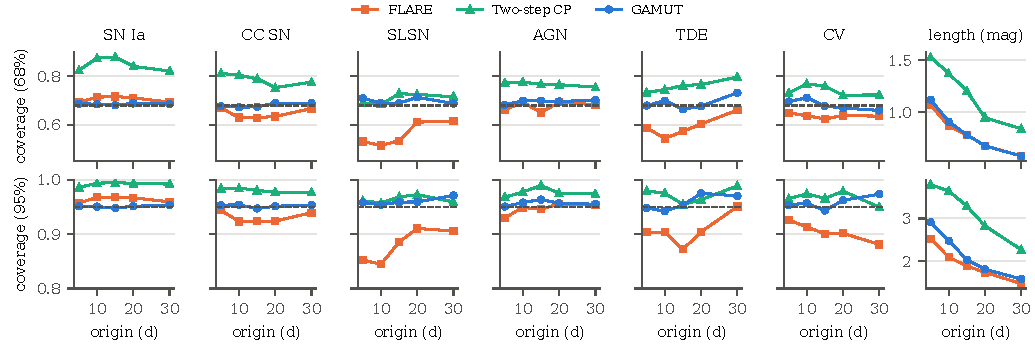
\includegraphics[width=0.92\textwidth]{figures/ztf_classes.pdf}
\vspace{-5pt}
\caption{ZTF-BTS per-class coverage and mean band width across forecast origins at 68\% (top) and 95\% (bottom) for FLARE, two-step CP, and \gamut{}. Dashed lines mark nominal coverage; right panels show mean band length in magnitudes.}
\label{fig:ztf}
\vspace{-4pt}
\end{figure*}

\paragraph{ZTF-BTS and Pre-Registered Held-Out Chunks.}
On ZTF-BTS (\cref{fig:ztf}), FLARE's 68\% SLSN and TDE coverage stays between \ZTFflareSLSNmin{} and \ZTFflareSLSNmax{}, whereas \gamut{} never falls more than \ZTFgamutMaxUnderSixtyeight{} (68\%) or \ZTFgamutMaxUnderNinetyfive{} (95\%) below nominal for any class at any origin at \ZTFWidthRatioSixtyeight{} and \ZTFWidthRatioNinetyfive{} times FLARE's width.
To bound post-inspection tuning (\cref{app:history}), we froze code checksums and ran once on untouched Wide-Fast-Deep transients from PLAsTiCC chunk 02 (20,760 objects, 12 classes; \cref{app:held}): FLARE is 0\% valid (worst class \HeldWorstFlareSixtyeight{} at 68\%), whereas \gamut{} is 100\% valid at all origins and levels at widths \HeldWidthGamutSixtyeight{} (68\%) and \HeldWidthGamutNinetyfive{} (95\%) versus \HeldWidthValidSixtyeight{} and \HeldWidthValidNinetyfive{} for conservative baselines (\HeldCellsGamutNinetyfive{} under-covered 95\% cells vs.\ 0.0 for two-step/max-class CP).
A second untouched WFD chunk 03 (20,475 objects; \cref{app:held}) confirms 100\% validity at widths \HeldBWidthGamutSixtyeight{} and \HeldBWidthGamutNinetyfive{} (FLARE: 0\%).

\subsection{Ablation, Synthetic, Strict-Split, and Closure Studies}
\begin{table}[t]
\centering
\caption{Ablations, aggregated over the six main benchmarks and all origins. Width is relative to full \gamut. Columns as in \cref{tab:main}.}
\label{tab:ablation}
\scriptsize
\setlength{\tabcolsep}{3pt}
\resizebox{\linewidth}{!}{%
\begin{tabular}{lccccc@{\hspace{6pt}}ccccc}
\toprule
 & \multicolumn{5}{c}{68\%} & \multicolumn{5}{c}{95\%} \\
\cmidrule(lr){2-6} \cmidrule(lr){7-11}
Variant & Val. & Worst & CCG & Cells & W. & Val. & Worst & CCG & Cells & W. \\
\midrule
\rowcolor{gray!12}\gamut{} (full) & 100 & 0.671 & 0.014 & 0.2 & 1.00 & 90 & 0.949 & 0.012 & 0.8 & 1.00 \\
\midrule
w/o C1: pooled forecaster & 100 & 0.675 & 0.017 & 0.1 & 1.04 & 85 & 0.952 & 0.015 & 0.7 & 1.03 \\
w/o C2: uniform posterior & 100 & 0.694 & 0.094 & 0.2 & 1.43 & 100 & 0.967 & 0.032 & 0.1 & 1.47 \\
w/o C2: argmax posterior & 100 & 0.698 & 0.089 & 0.0 & 1.38 & 100 & 0.960 & 0.029 & 0.0 & 1.35 \\
w/o C2 calibration (raw $\tilde p$) & 100 & 0.672 & 0.014 & 0.1 & 1.01 & 90 & 0.948 & 0.012 & 0.6 & 1.00 \\
w/o C3: posterior mixture & 0 & 0.516 & 0.068 & 15.1 & 0.86 & 0 & 0.862 & 0.026 & 10.2 & 0.73 \\
w/o C3: prior-ratio weights & 100 & 0.686 & 0.175 & 0.1 & 1.45 & 100 & 0.964 & 0.030 & 0.0 & 1.17 \\
fixed lead bins (no merging) & 100 & 0.671 & 0.015 & 0.1 & 1.01 & 95 & 0.946 & 0.013 & 0.2 & 1.03 \\
\gamut{} (split calibration) & 100 & 0.745 & 0.096 & 0.0 & 1.33 & 100 & 0.968 & 0.028 & 0.1 & 1.29 \\
\bottomrule
\end{tabular}}
\end{table}


\paragraph{Ablations and Synthetic Suite.}
In \cref{tab:ablation}, uniform or argmax posteriors keep validity via \textbf{C3} but widen bands by \AblWidthUniform{} and \AblWidthArgmax{}; dropping \textbf{C3} collapses 68\% validity to \AblValidMixtureSixtyeight{} (worst \AblWorstMixtureSixtyeight{}), and static inverse-prior weights add \AblWidthBalanced{} width.
Dropping \textbf{C1} shifts real-benchmark width by \AblWNoConeSixtyeight{}/\AblWNoConeNinetyfive{} (95\% validity \MainValidGamutNinetyfive{}$\to$\AblValidNoConeNinetyfive{}) where early prefixes look similar across classes, but \textbf{C1} cuts width by \AblConeSynSixtyeight{}/\AblConeSynNinetyfive{} on synthetic data with distinct class trajectories, where \gamut{} approaches the oracle band within \SynOracleGapSixtyeight{}/\SynOracleGapNinetyfive{} versus \SynOracleGapValidSixtyeight{}/\SynOracleGapValidNinetyfive{} for valid baselines (\cref{app:synthetic}).
Temperature scaling changes real width little (\AblWRawSixtyeight{}, \AblValidRawNinetyfive{} valid at 95\%) but saves \AblRawKtwoSixtyeight{}/\AblRawKtwoNinetyfive{} at $\kappa=2$.
Without leave-one-object-out scoring, day-20 ZTF CV coverage drops to \AblWorstNoLooZTF{} (95\% validity \AblValidNoLooNinetyfive{}); one horizon-wide threshold lets a ZTF cell hit \AblOneThreshWorstCell{}; and validation sweeps shift worst-class coverage by $\le$\HyperMaxWorstChange{} and width by $\le$\HyperMaxWidthChange{} aside from 5 dual steps raising ECG5000 CCG from \HyperDualFiveCCGFrom{} to \HyperDualFiveCCGTo{} (\cref{app:hyper}). Fixed bins slightly edge adaptive merging on 95\% test folds (\AblValidFixedBinsNinetyfive{} valid, \AblWFixedBinsSixtyeight{}/\AblWFixedBinsNinetyfive{} width), but we retain validation-chosen merging (\HyperFixedBinsWidthMin{}--\HyperFixedBinsWidthMax{} narrower on validation) and object-level units (\cref{thm:valid}).

\paragraph{Strict Three-Way Split.}
Rotating three base-training folds, one calibration fold, and one test fold on ZTF-BTS satisfies \cref{thm:valid} (\cref{tab:strictsum}, \cref{app:cert}).
Across all \StrictNOrigins{} origins, FLARE is 0\% valid, whereas \gamut{} is 100\% valid at widths \StrictWidthGamutSixtyeight{} (68\%) and \StrictWidthGamutNinetyfive{} (95\%) versus \StrictWidthTwoStepSixtyeight{}--\StrictWidthMDCPSixtyeight{} and \StrictWidthTwoStepNinetyfive{}--\StrictWidthMDCPNinetyfive{} for always-valid baselines.
Certified \emph{\gamut{} (strict split)} achieves 100\% empirical validity at widths \StrictWidthCertSixtyeight{} and \StrictWidthCertNinetyfive{}; at 95\%, full-fold \gamut{} is wider because 19--39-object classes remain active with near-zero risk budget, whereas Half-$B$ size screening ($n^B_{c,b}\ge19$) certifies SN~Ia and CC~SN while excluding SLSN, AGN, TDE, and CV.

\paragraph{Next-Observation Set Closure.}
To predict whether one next-night detection narrows FLARE's 90\% classification set to a singleton, replacing FLARE's argmax-routed fixed-scatter Gaussian draws with \textbf{C1} empirical-residual draws, \textbf{C2} mixing, and inductive Venn--Abers \citep{vovk2014venn} cuts test Brier score by \CloFiveBrierGainVA{} (day 5) and \CloTenBrierGainVA{} (day 10) against Venn--Abers-recalibrated FLARE and lifts AUC (\CloFiveAUCDep{}$\to$\CloFiveAUCOurs{}, \CloTenAUCDep{}$\to$\CloTenAUCOurs{}) at matching ECE (\cref{app:closure}).
Uncalibrated, it meets FLARE's $\pm0.10$ five-bin tolerance in \CloFiveProfOursRaw{} and \CloTenProfOursRaw{} bins versus \CloFiveProfDep{} and \CloTenProfDep{}.
A pooled empirical-residual control gives Brier \CloFiveBrierPooled{} and \CloTenBrierPooled{}, showing that the learned next-point law rather than class mixing drives the gain, while small day-10 SLSN slices remain noisy.
